% This is sigproc-sp.tex -FILE FOR V2.6SP OF ACM_PROC_ARTICLE-SP.CLS
% OCTOBER 2002
%
% It is an example file showing how to use the 'acm_proc_article-sp.cls' V2.6SP
% LaTeX2e document class file for Conference Proceedings submissions.
% ----------------------------------------------------------------------------------------------------------------
% This .tex file (and associated .cls V2.6SP) *DOES NOT* produce:
%       1) The Permission Statement
%       2) The Conference (location) Info information
%       3) The Copyright Line with ACM data
%       4) Page numbering
%
%  However, both the CopyrightYear (default to 2002) and the ACM Copyright Data
% (default to X-XXXXX-XX-X/XX/XX) can still be over-ridden by whatever the author
% inserts into the source .tex file.
% e.g.
% \CopyrightYear{2003} will cause 2003 to appear in the copyright line.
% \crdata{0-12345-67-8/90/12} will cause 0-12345-67-8/90/12 to appear in the copyright line.
%
% ---------------------------------------------------------------------------------------------------------------
% It is an example which *does* use the .bib file (from which the .bbl file
% is produced).
% REMEMBER HOWEVER: After having produced the .bbl file,
% and prior to final submission,
% you need to 'insert'  your .bbl file into your source .tex file so as to provide
% ONE 'self-contained' source file.
%
% Questions regarding SIGS should be sent to
% Adrienne Griscti ---> griscti@acm.org
%
% Questions/suggestions regarding the guidelines, .tex and .cls files, etc. to
% Gerald Murray ---> murray@acm.org
%
% For tracking purposes - this is V2.6SP - OCTOBER 2002

\documentclass{acm_proc_article-sp-sigmod09}
\usepackage{url}
\usepackage{algorithm}
\usepackage[noend]{algpseudocode}
\usepackage{float}
\begin{document}
\algnewcommand\algorithmicforeach{\textbf{for each}}
\algdef{S}[FOR]{ForEach}[1]{\algorithmicforeach\ #1\ \algorithmicdo}
%
% --- Author Metadata here ---
\conferenceinfo{Data Mining}{Academic year 2018-2019}
%\setpagenumber{50}
%\CopyrightYear{2002} % Allows default copyright year (2002) to be over-ridden - IF NEED BE.
%\crdata{0-12345-67-8/90/01}  % Allows default copyright data (X-XXXXX-XX-X/XX/XX) to be over-ridden.
% --- End of Author Metadata ---

\title{Frequent itemset mining in tree-like sequences of complex objects}
\numberofauthors{2}
\author{
\alignauthor
Nicol\`o Pomini\\
       \affaddr{Mat. 203319}\\
       \affaddr{University of Trento, Trento}\\
       \affaddr{nicolo.pomini@studenti.unitn.it}
\alignauthor
Marco Merlin\\
       \affaddr{Mat. 205263}\\
       \affaddr{University of Trento, Trento}\\
       \affaddr{marco.merlin@studenti.unitn.it}
}
%
\maketitle
\begin{abstract}
Data mining is a branch of computer science which studies how to extract or infer useful information from data which may or may not seem to have any. Very often the kind of information that are tried to be extracted are correlations in the data which may suggest some kind of \emph{trends}. Finding these \emph{trends}, or patterns, means that given the appearance of an element in the data, we could predict the appearance of another element. In this paper are discussed and described the methods, the algorithms used and the results obtained during the implementation of a data mining applications for frequent patterns in tree-like sequences of complex objects. These tree-like structures are composed of nodes which can contain several attributes. The domain of the attributes is not relevant as the application should find the patterns independently from the context which they represent. The patterns may present very complex structures which may involve many attributes in one node implying many other attributes in a subsequent node. Such a task brings many challenges among which there are time constraints as these kind of tasks can grow very quickly in complexity.
\end{abstract}

\terms{Data mining}

\keywords{Tree mining, frequent itemset mining}

\section{Introduction}
We live in a world full of data. It is generated in several ways: humans produce data every day, for example using the Internet and the social media; machine generates much more data than the former, for example creating logs or communicating with each other; scientific world is another important producer, but also IoT devices, or health care systems and real time information management. There are endless contributor to the generation of heterogeneous forms of data.

Nowadays data is very easy to retrieve: let us think about the Internet scenario, where every click, every scroll, and every page visited can be tracked: a single user can produce -- without his knowledge, maybe -- dozens of records in a really small amount of time, and these records are saved into a database somewhere. The real challenge is to explore this huge amount of data, to turn it into useful and meaningful information. Many firms may have stored all possible and imaginable data since their foundation, and inside of it there is a potential information mine: for example, the secret of how to make the production of a certain good more efficient, or the preferences of their customers coming from a specific geographic location. Very often the goal of what to search in data is not known, the only constraint is to get something useful.

The latter is the scenario of data mining: extract information from a source of data, without knowing exactly what to search for or what to expect. This project explores one possible application of data mining techniques, where data has a particular but flexible structure, and the results are not predictable.

This report is about the project for the \emph{data mining} course offered by the department of information engineering and computer science\footnote{\url{www.disi.unitn.it}} of the university of Trento. The report is organized as follows: \dots

\section{Problem description}
In many scenarios, applications produce records that contain several fields, and these fields are not always indepentent, but the appearence of one may mean the appearence of some others. For example, a list of purchases in a shop can contain similar patterns, or a call made by a web service to some external RESTful services may lead to further calls to other services. Other similar examples can be the flows of exploration of a website, or of a chain of websites, or public administration processes, like the analysis of cases where people ask permissions to restructure buildings or facilities. 

These examples share a common property: when executed by several people, they produce some \emph{paths} that are more frequent that others. A path can be a list of web pages ordered by visit, or a set of RESTful service calls made by a server, in order of execution, or the purchase of a precise item that leads to some other purchase. For example, buying a toothbrush is likely to purchase also some toothpaste: if this was the case, observing the list of purchases of a shop, and considering those cases where the former item is bought, it would be easy to find also the latter product. This is an example of a \emph{frequent pattern}.

The goal of this assignment is, given a set of objects connected each other and representing some action in a possible scenario equal or similar to those listed above, find these paths that are more frequent that the others. 

The reality modelled by this problem is made of \emph{records}, where a single record is a possible action performed in a concrete instance of the problem: a RESTful service request or response, the purchase of an item, a click on a button inside a web page, ect. One record is a list of key-value attributes: for example, in a HTTP request/response scenario, the possible attributes of the record can be the IP addresses of the sender and of the recipient, the timestamp of the request, the type of request (e.g. GET, POST), etc. 

The records are organized into \emph{transactions}, where a transaction is a set of ordered records, structured as a tree. This means that inside of a transaction there is a main record -- the root -- that eventually gives origin to other records, who themselves can generate other records and so on. Being a tree means that each record has at most one parent record -- another record that originated the current one -- and only if the considered record is the root of a transaction it has not a parent. Furthermore, this constraint allows not to have loops inside transactions. A transaction can be a list of RESTful service calls made by some server to fulfill a user's request, or a list of items bought by a customer.

Given a set of transactions, the expected output is a set of (sub)transactions that appear frequently inside the original ones.

\section{Approach description and similar problems}
\label{sec:general}
The naive approach to solve this problem consists in generating all the possible combinations of attributes of records of all the transactions, to observe how many times each combination appears, and to select those apprearing at least a certain number of time $f$. By definition, this approach has a high computational complexity, since the number of combinations grows exponentially with the number of transactions and the number of possible values of the attributes of the records.

Furthermore, a pattern has a tree structure, and it can be developed in three different ways.
\begin{itemize}
\item Horizontal -- which means that the pattern is made of a single record, with more than an attribute involved. This kind of pattern is a sort of a logical implication regarding two or more attributes in the same record, where the existence of a certain value implies the existence of some other values in the same record. Referring to Figure~\ref{fig:transaction}, the only possible horizontal pattern is $\{a_1 \colon v_1, a_2 \colon v_2\}$.
\item Vertical -- when the pattern involves more than one record, and for each record one field is concerned, creating a tree structure. In this case, at least two records must be used to create such a pattern, otherwise any frequent value -- like every \texttt{tid} -- would be a pattern. The records in which appear a value belonging to the pattern do not have to be contiguous: in fact, it is possible to have a pattern made of three nodes -- for example $x, y, z$, with $x$ parent of $y$ and $y$ parent of $z$, where the existance of a value in $x$ implies the existance of a value in $z$, with any possible value in $y$. Referring to Figure~\ref{fig:transaction}, the possible vertical patterns are $\{a_1 \colon v_1, a_3 \colon v_3\}$, $\{a_2 \colon v_2, a_3 \colon v_3\}$, $\{a_1 \colon v_1, a_4 \colon v_4\}$, $\{a_2 \colon v_2, a_4 \colon v_4\}$, but also $\{a_3 \colon v_3, a_4 \colon v_4\}$. The latter is an example of a non-contiguos pattern: the parent has any value, and the two children have a value that implies the other one.
\item Horizontal and vertical -- the case of a vertical pattern, in which the records can have more than one attribute involved in the pattern. Referring to Figure~\ref{fig:transaction}, they can be $\{a_1 \colon v_1, a_2 \colon v_2, a_3 \colon v_3\}$, $\{a_1 \colon v_1, a_2 \colon v_2, a_4 \colon v_4\}$ or $\{a_1 \colon v_1, a_2 \colon v_2, a_3 \colon v_3, a_4 \colon v_4\}$.
\end{itemize}

This means that a pattern can have a very complex structure, and it can involve several records spread across the whole transaction.

The idea of the developed solution for this problem is to reduce the numbers of possible combinations of attributes of records to generate, using a well-known problem that is similar but easier to the current one, the \emph{frequent itemsets} problem. The proposed solution flattens the tree structures into a list of strings, where a single string is the concatenation of an attribute key with its value, and for each tree -- a single transaction -- a list containing all the concatenations of all the records belonging to the tree is generated. 

\newdef{definition}{Definition}
\begin{definition}
Given a transaction $t$, its flattered representation -- $flattered(t)$ -- is a set of strings defined in the following way:
\[
\{r.a_{key} \oplus r.a_{value} \quad \forall r \in records(t) \quad \forall a \in attributes(r) \}
\]
where $records(t)$ is the list of records belonging to the transaction $t$, $attributes(r)$ are all the attributes in the record $r$, and $\oplus$ is the string concatenation operation.
\end{definition}

Therefore, $n$ transactions are flattened into $n$ lists of strings, and these list are given to the frequent itemset miner algorithm, which returns a list of tuples of attributes, where each tuple is a recurrent list of attributes inside all the transactions. Strings of concatenated key-values attributes are used because they allow to distinguish easily all the possible combinations of values for each attribute.

This approach allows to prune the space of possible frequent patterns: in fact, if a combination of attributes does not belong to the frequent itemsets, it is not a frequent pattern.

\newtheorem{theorem}{Theorem}
\begin{theorem}
The combinations of attributes that do not appear in the result of the frequent itemset algorothm do not form any frequent pattern.
\end{theorem}

\begin{proof}
Let us prove the theorem by contradiction. Let assume that a pattern $p$ is frequent, and its $flattered(p)$ does not appear entirely in the resulting frequent itemsets. This means that its attributes do not appear frequently in the whole set of transaction, and thus it is not possible to create a pattern with these attributes that is frequent among all the transactions. This means that $p$ is not frequent, and this is a contradiction with the initial assumption.
\end{proof}

Starting from the frequent itemsets, the frequent patterns are searched for. Unfortunately, the result of the frequent itemsets does not give any information about the structure of the pattern, so the only available knowledge is that the pattern is made of at least those attributes.

There are similar problems but different from this one, and now a brief description of them is provided. Finally, some assumptions on the current problem are stated.

\subsection{Frequent item-sets problem - Association rules}
\label{sec:freqitemset}
In this scenario, there exists records very similar to those in the problem descibed in this report. In fact, also here a record can have an arbitrary number of attributes, which are called \emph{items}. Given a list of records, the goal of this problem is to find sets of items that appear frequently inside records. Usually, the minimum frequency of appearance to consider a set of items as a frequent itemset is a parameter of the problem, and often it is express as a fraction of the number of records that contain the set with respect to the total number of records.

This problem is computed iteratively, starting with itemsets of cardinality equals to 2, and trying to growing the size of the sets until there are no more frequent sets. The idea is to use the $k$-frequent itemsets -- those itemsets whose size is equal to $k$ -- to build valid $k + 1$-frequent itemsets.

There are several approach to this problem, like the \emph{A priori} or the \emph{PCY} algorithms, which optimize the use of memory and the number of disk reads.

An extension of this problem is the \emph{Association rules} mining, where, instead of simple sets of attributes, logic implication rules are searched for -- in the form $\{a_i, \dotsc, a_k\} \implies \{a_j, \dotsc, a_l\}$. In the previous case, the order with which the attributes are found inside a record does not matter, since it is only necessary that they appear together; in this case, instead, the order matters: in fact, the expressions $A \implies B$ and $B \implies A$ are different.

In the literature, these problems are well known, and several publications about them exist, such as \cite{agrawal1994fast, ivancsy2006time, rakesh1993mining, brin1997dynamic}.

This scenario is not sufficient for the main problem considered in this report, because the former has a lack of structure in the data. The proposed view is flattened, and it is not possible to infer tree like structure froms simple sets of attributes. Anyway, our approach is based on these problems, since -- as stated in Theorem~1 -- the attributes of a frequent pattern in a tree scenario belong to a frequent itemset of the flattened representation of the trees.

\subsection{Frequent subtrees discovery}
There are several publications that deal with the discovery of frequent sub-structures inside structured data. In case data is structured as a sequence, the problem and the most common techniques to resolve it are briefly explained in Section~\ref{sec:freqitemset}.

Data can have a more complex structures than a linear sequences: it can be organized in trees or graphs. The nature of the main problem of this report belongs to these cases. The state of the art offers several approaches to mine the frequent sub-structures inside complex structures of data.

In case data is a graph, an efficient algorithm based on the adjancy matrix of the graph itself is proposed in \cite{inokuchi2000apriori, kuramochi2001frequent}, inspired by the A-Priori algorithm for the frequent itemset problem. Some other publications, such as \cite{zaki2002efficiently}, deal with data organized in trees, or in a set of trees -- a forest. At first sight, this might seem to be exacly the same problem discussed in this report, but there is a huge difference: in \cite{zaki2002efficiently}, each node of a tree has one and only one \emph{label} -- an attribute, such as an integer or a string, stored in the node. Instead, our problem is about nodes that can contain an arbitrary number of attributes -- in this case \emph{labels}. Having only one label per node simplifies a lot the problem, since the possible combinations of attributes between two nodes are much less than those in the main problem discussed in this report.

Finally, there is an approach to solve the frequent itemset problem explained in Section~\ref{sec:freqitemset} building a tree, and finding the frequent subtrees in it. This technique is explained in \cite{han2004mining}, but again, it is not useful for our problem. In fact, in this scenario the data is flat -- organized in lists of \emph{items} -- and furthermore the tree generated by the considered algorithm is made by nodes having only a single label.

\subsection{Assumptions}
\label{sec:assumptions}
For the sake of simplification, some assumption exists.

All the records contain at least four attributes: the \texttt{rid} to identify the record; the \texttt{tid} to recognize to which transaction the record belongs; a \texttt{parent} field, containing the \texttt{rid} of the parent record -- which can be empty in case the considered record is the root of a transaction; at least another attribute, which can have any name and any type. The latter kind of attribute is called \emph{generic attribute}. The patterns are searched for only on \emph{generic attributes}, and not on the other three types, which do not create any pattern since they are used to describe the structure of the transactions.

\begin{definition}
A \emph{generic attribute} is any attribute of a record which is not the \texttt{rid}, the \texttt{tid} or the \texttt{parent} attributes. These attributes represent the features of each record, and the patterns are made of \emph{generic attributes}.
\end{definition}

All the records are assumed to have the same attributes -- some of them may be empty, to make the organization of the data easier. This contraint does not cause any loss of generality: in fact, in case the records are desired to be composed by a different number (and type) of attributes, it is sufficient to provide to each record all the attributes, living some of them empty.

The data is assumed to be organized in a matrix $M \in \Sigma^{n * d}$, where $\Sigma$ is the dictionary from which the values of the attributes belong to -- it can be a finite subset of $\mathbb{N}$, or a set of strings -- $n$ is the number of records, and $d$ the number of attributes per record. Furthermore, a vector of strings $\boldsymbol{a}$ is expected, containing the names of the attributes.

Without loss of generality, all the names and the values of the attributes of a record are assumed to be strings -- since every object can be represented by a string and built from a string.

\section{Problem statement}
A record $\boldsymbol{r}$ is a tuple, in the form $<a_1 \colon v_1, a_2 \colon v_2, \text{\dots}, a_n \colon v_n>$, where a pair $a_i \colon v_i$ represents an attribute-value relationship, where $a_i$ is the attribute and $v_i$ the value. These pairs can contain any kind of data, such as numbers or strings. To identify a record, is assumed that each one has an attribute called \emph{record id}, or \texttt{rid} for short.

A transaction $\boldsymbol{T}$ is a set of records $\{\boldsymbol{r_1}, \boldsymbol{r_2}, \text{\dots}, \boldsymbol{r_m}\}$ that forms a tree structure, which means that a transaction has a root record, which has some \emph{children records}, which in turn have some other children, and so on. To identify the transaction in which each record belongs, it is assumed that every record has an attribute called \emph{transaction id}, or \texttt{tid} for short.

\begin{figure}
\centering
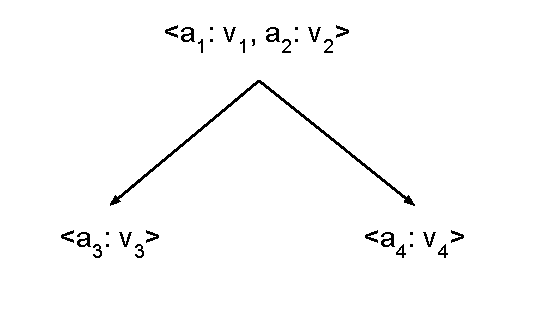
\epsfig{file=PatternExample.pdf}
\caption{An example of transaction, made of three records.}
\label{fig:transaction}
\end{figure}

Let us define a pattern.
\begin{definition}
A pattern is a set of ordered attributes and values belonging to possibly different records in the same transaction. In other words, a pattern is any ordered subset of $\bigcup\limits_{i=1}^{n} \bigcup\limits_{j=1}^{m} \boldsymbol{r_i}<a_j \colon v_j>$, where the ordering is given by the hierarchy of the transaction. For example, in Figure~\ref{fig:transaction} some possible example of pattern are $\{a_1 \colon v_1, a_3 \colon v_3\}$ or $\{a_2 \colon v_2, a_3 \colon v_3\}$, but not $\{a_4 \colon v_4, a_1 \colon v_1\}$, beacuse the latter breakes the hierarchic order.

By definition, since a transaction is structured as a tree, also a pattern is a tree. This means that a pattern must respect the constraints given by the nature of the data structure: each node has at most one parent node, and there are no loops inside the tree, which means that the edges of the tree are meant to be directed from the parent towards the child node.
\end{definition}

Given a set of transactions, the goal is to identify patterns of attributes that are frequent, which means transaction that appear at least a given number of time $f$.

\section{Algorithms}
The procedure to mine the frequent patterns inside the transactions follows these steps: first of all, the input file is scanned and organized into some data structures; secondly, each transaction is submitted to the frequent itemsets algorithm; thridly, each frequent itemset is analyzed in each transaction, searching if the itemset appears in some ways inside the transaction; finally, the found pattern are counted, and those above the given threshold $f$ are kept and displayed as frequent.

In this section the various parts are described in details.

\subsection{Input parsing and data organization}
As said in Section~\ref{sec:assumptions}, the expected input is composed by a matrix $M \in \Sigma^{n * d}$, where $\Sigma$ is the dictionary from which the values of the attributes belong to -- it can be a finite subset of $\mathbb{N}$, or a set of strings -- $n$ is the number of records, and $d$ the number of attributes per record. In addition to that, a vector of strings $\boldsymbol{a}$ is needed, containing the names of the attributes. Of course at least three attributes -- \texttt{rid}, \texttt{tid}, \texttt{parent} -- must be part of $\boldsymbol{a}$. Furthermore, an integer threshold $f$ is needed, to decide how many times a frequent pattern has to appear at least.

At the beginning, $M$ is scanned by its rows, and each record (a single row $i$ of the matrix) is saved into a dictionary: the key of a record is its \texttt{rid}, and the content is a set of pairs $<k_j \colon v_j>$, where $k_j = \boldsymbol{a}_j$ and $v_j = M[i,j]$. In this way, given the \texttt{rid}, it is very easy and fast to retrieve the entire record. The dictionary is called $records$. The algorithm to populate this dictionary is trivial, and for this reason is omitted from the report. It is assumed that the dictionary data structure, with a method to add an object giving its key -- $add(key, value)$ -- and a method to search by key -- $lookup(key)$ -- exists.

After that, the attributes of the records are analyzed, to reconstruct the transactions. To do so, a data structure -- called Tree --- is used: it is a simple tree made by nodes, where a node can have an arbitrary number of children. This data structure is defined in Table~\ref{tab:tree}. As can be seen, this data structure is needed to keep track of the structure and the hierarchy between nodes belonging to the same transaction. A node having the parent attribute set to the \texttt{null} type -- $\bot$ -- is a root of a transaction.

\begin{table}[H]
\centering
\begin{tabular}{|ll|} \hline
\textbf{Tree} & \\ \hline
\textbf{parent} & Tree \\ \hline
\textbf{children} & Tree[] \\ \hline
\textbf{rid} & string \\
\hline\end{tabular}
\caption{Tree object definition.}
\label{tab:tree}
\end{table}

To build the transaction, two scans of the dictionary $records$ are needed: the first one to create a node for each record, the second one to assign the degrees of kinship between nodes. In particular, during the second iteration, every node is checked to see if its parent has a value, or it is set to $\bot$: in the first case, it means that the node has a parent, and so its parent is set, and in its parent the node is added as a child; in the second case, it means that the node is a root of a transaction, and so the node is added to a dictionary of treees $roots$. This process is described in the Algorithm~\ref{build_trees}, which returns the dictionary of trees containing the root node of each transaction.

\begin{algorithm}
\caption{Construct the transactions from the dictionary of records $records$.}
\label{build_trees}
\begin{algorithmic}[1]
\Function{generateTrees}{Dictionary $records$}
\State $roots \gets new Dictionary()$
\State $nodes \gets new Dictionary()$
\For{$rid \in records$}
	\State $node \gets new Tree()$ 
	\State $node_{rid} \gets rid$
	\State $nodes.add(rid, node)$
\EndFor
\For{$rid \in records$}
	\State $parent \gets records.lookup(rid)_{parent}$
	\If{$parent = \bot$}
		\State $roots.add(rid, nodes.lookup(rid))$
	\Else
		\State $child \gets records.lookup(rid)$
		\State $parent_{children} \gets parent_{children} \cup \{child\}$
		\State $child_{parent} \gets parent$
	\EndIf
\EndFor
\Return $roots$
\EndFunction
\end{algorithmic}
\end{algorithm}

\subsection{Frequent itemsets in transactions}
Once the input is parsed and the tree structures are built, it is time to apply the frequent itemsets mining algorithm, to search for tuples of attributes that will be the starting point of the frequent pattern mining. As explained in Section~\ref{sec:general}, this approach allows to optimize the number of patterns to search inside the transaction: instead of trying all the possible combinations of attributes, a frequent itemset mining is applied to filter some combinations that for sure would not give any frequent pattern.

The frequent itemset mining algorithm is well known, and it is widely described in \cite{agrawal1994fast}. For this description, it is assumed to have a function $frequentItemsets(String[][] itemsets, float confidence)$ that takes a list of list of strings, and a floating point number representing the minimum confidence needed to consider an itemset as frequent. This function returns a set if tuples, where each tuple contains an arbitrary number of attributes.

To transform a transaction -- whose structure is a tree -- to a list of strings, the function $flattered(Tree t)$ is used. This function has to be able to flatten the tree structure, but also to distinguish between attributes with the same name but with different values. To do so, the name and the value of each attribute of each record are concatenated together, putting in between a special string " = ". For example, if the record $r_1$ has the attribute $<a \colon 1>$ and the record $r_2$ the attribute $<a \colon 2>$, the string version of their attribute is, respectively, "a = 1" and "a = 2". Let us define formaly such function. An important osservation is that the frequent itemsets algorithm works with sets of attributes, so the order with which a transaction is traversed to create its flattened version is indifferent. The procedure is described in Algortihm~\ref{flatten}, which is a wrapper function for the Algorithm~\ref{flattenrec}.

\begin{algorithm}
\caption{Create the flattened version of a transaction.}
\label{flatten}
\begin{algorithmic}[1]
\Function{flatten}{Tree $t$, Dictionary $records$}
\State $itemsets \gets new String[]$
\State $flattenRec(t, records, itemsets)$ \\
\Return $itemsets$
\EndFunction
\end{algorithmic}
\end{algorithm}

\begin{algorithm}
\caption{Recursive function to create the flattened version of a transaction.}
\label{flattenrec}
\begin{algorithmic}[1]
\Function{flattenRec}{Tree $t$, Dictionary $records$, String[] $itemsets$}
\State $record \gets records.lookup(t_{rid})$
\For{$tuple \in record$}
	\State $s \gets tuple_{key} \oplus \text{" = "} \oplus tuple_{value}$
	\State $itemsets \gets itemsets \cup \{s\}$
\EndFor
\For{$child \in t_{children}$}
	\State $flattenRec(child, records, itemsets)$
\EndFor
\EndFunction
\end{algorithmic}
\end{algorithm}

Finally, all the transaction are flattened, and the resulting matrix of strings -- where on the rows there are the various transactions, and on the columns the concatenated attributes -- is given as input to the frequent itemsets algorithm. This can be seen in Algorithm~\ref{freqitemset}.

\begin{algorithm}
\caption{Flat the transaction and compute the frequent itemsets.}
\label{freqitemset}
\begin{algorithmic}[1]
\Function{getFrequentItemsets}{Tree[] $transactions$, Dictionary $records$, float $confidence$}
\State $globalItemsets \gets new String[][]$
\For{$t \in transactions$}
	\State $flat \gets flatten(t, records)$
	\State $globalItemsets \gets globalItemsets \cup \{flat\}$
\EndFor
\Return $frequentItemsets(globalItemsets, confidence)$
\EndFunction
\end{algorithmic}
\end{algorithm}

\subsection{Frequent pattern mining}

\subsection{Pattern count}
describe eq and hash of trees \dots

\section{Implementation}
\dots

\section{Experiments}
\dots

\section{Conclusions}
\dots

%\end{document}  % This is where a 'short' article might terminate
%
% The following two commands are all you need in the
% initial runs of your .tex file to
% produce the bibliography for the citations in your paper.
\bibliographystyle{abbrv}
\bibliography{sigproc}  % sigproc.bib is the name of the Bibliography in this case
\end{document}
